\chapter{Background} \label{chp:background}
    To best understand the work done in this thesis, some background information on laser-thermal propulsion is provided in this chapter. This is an abridged version of the literature review~\cite{duplayReviewLaserThermalPropulsion2022} written before starting this thesis, which can be consulted for an in-depth study of past literature. The working principle of LTP will first be discussed, including a brief discussion of DEP and alternate concepts that also fall under the LTP category. A thorough discussion of LSP, the physics powering the laser-plasma LTP thruster, will then be given. Finally, an overview of the experimental work done on both LSP and LTP will be provided.

    \added{Although hydrogen is the preferred candidate for LTP propellant to maximize specific impulse (as implied by \autoref{eq:isp}), many LSP studies have also considered other gases, usually noble gases. Discussion of the literature will include such studies, specifically those on argon LSP, as it is the working fluid studied in this project. The rationale for choosing argon as propellant will be discussed at the end of this chapter, after}\deleted{This chapter will then end by} stating research objectives\deleted{ for this thesis,} derived from the findings of the literature review\deleted{ summarized here}.

    \section{Working principle} \label{sec:background_principle}
        LTP is a directed-energy propulsion concept, a class of propulsion systems where energy is beamed to a spacecraft, usually using a laser\footnote{Theoretically, a fully-contained LTP system could be used aboard a spacecraft, but this would not leverage the main benefit of laser propulsion, i.e., high propulsion system power for a low mass penalty}. This energy is then used for propulsion either directly or through an intermediate conversion process. This allows the spacecraft to forego much of its power and propulsion system mass, increasing its propellant or payload mass budget. Some applications of DEP, such as lightsails, even bypass the rocket equation altogether, making them a promising avenue for interstellar missions, as shown by \textcite{lubinRoadmapInterstellarFlight2016a}. \citeauthor{lubinRoadmapInterstellarFlight2016a} proposes modular, scalable fiber-laser arrays operating at \qty{1064}{nm} to beam the required MW to GW of power necessary to propel interplanetary and interstellar spacecraft. This specific laser wavelength transmits with virtually no losses through the atmosphere (\textcite{geminiobservatorySites2020}), and perturbations caused by atmospheric turbulence can be readily corrected using adaptive optics technology already in use in astronomy, as discussed by \textcite{eckelLaserPropulsionSystems2008, hettelBeamPropagationSimulation2021}. \added{The choice of fiber-pumped lasers for DEP is also driven by economics: \textcite{lubinRoadmapInterstellarFlight2016a} discusses that the cost and size of fiber-pumped laser amplifiers has been driven down exponentially thanks to the growing use of fiber-optics in the telecommunications industry. This affordability enables the practical, scalable, and modular construction of large and high-power laser arrays in a manner not possible for a single monolithic laser.}

        \emph{Laser-thermal propulsion} itself encompasses several concepts where the laser is used to energize a propellant stored aboard the spacecraft. \textcite{kantrowitzRelevanceSpace1971} first proposed this idea as a way to reduce launch costs. Such concepts include pulsed concepts that ablate solid propellant or cause laser-supported detonations, as studied by \textcite{myraboPowerBeamingTechnologyLaser1984}, or laser heat-exchanger systems, as proposed by \textcite{kareLaserpoweredHeatExchanger1995}. 
        
        The present work focuses on continuous-wave (CW) laser-plasma propulsion, proposed by \textcite{noredApplicationHighPower1976} and studied in detail by \textcite{keeferLaserSustainedPlasmas1989}: as illustrated in \autoref{fig:overview}, a continuous laser is used to power a laser-sustained plasma (LSP)\footnote{This physical phenomenon is also referred to as \emph{optical plasmatron}, \emph{light spark}, \emph{continuous optical discharge} (COD), or \emph{laser-supported combustion} (LSC) wave in the literature.} core within a thrust chamber (\autoref{fig:overview_chamber}). This plasma absorbs laser energy and redistributes it to the propellant gas via conduction and radiation. The heated propellant is then expelled through a high-area ratio nozzle, like any other vacuum-optimized thermal rocket engine. It should be highlighted that although the LSP can attain temperatures of \qtyrange{20000}{30000}{K} (\textcite{noredApplicationHighPower1976}), it is thought to be relatively small compared to the thrust chamber size. The heat from the LSP core is distributed to the cooler gas flowing past it, resulting in a bulk propellant temperature at the nozzle inlet of ``only'' 10~000~K (\textcite{duplayDesignRapidTransit2022}). As will be discussed further in \autoref{sec:background_lsp}, the LSP core's position and size is easily controlled by the laser beam geometry (\textcite{keeferLaserSustainedPlasmas1989}), requiring no additional confinement mechanisms (such as the ones seen in fusion propulsion concepts) to separate the plasma from the chamber walls. 
        
        \begin{figure}[t]
            \centering
            \begin{subfigure}[t]{0.64\textwidth}
                \centering
                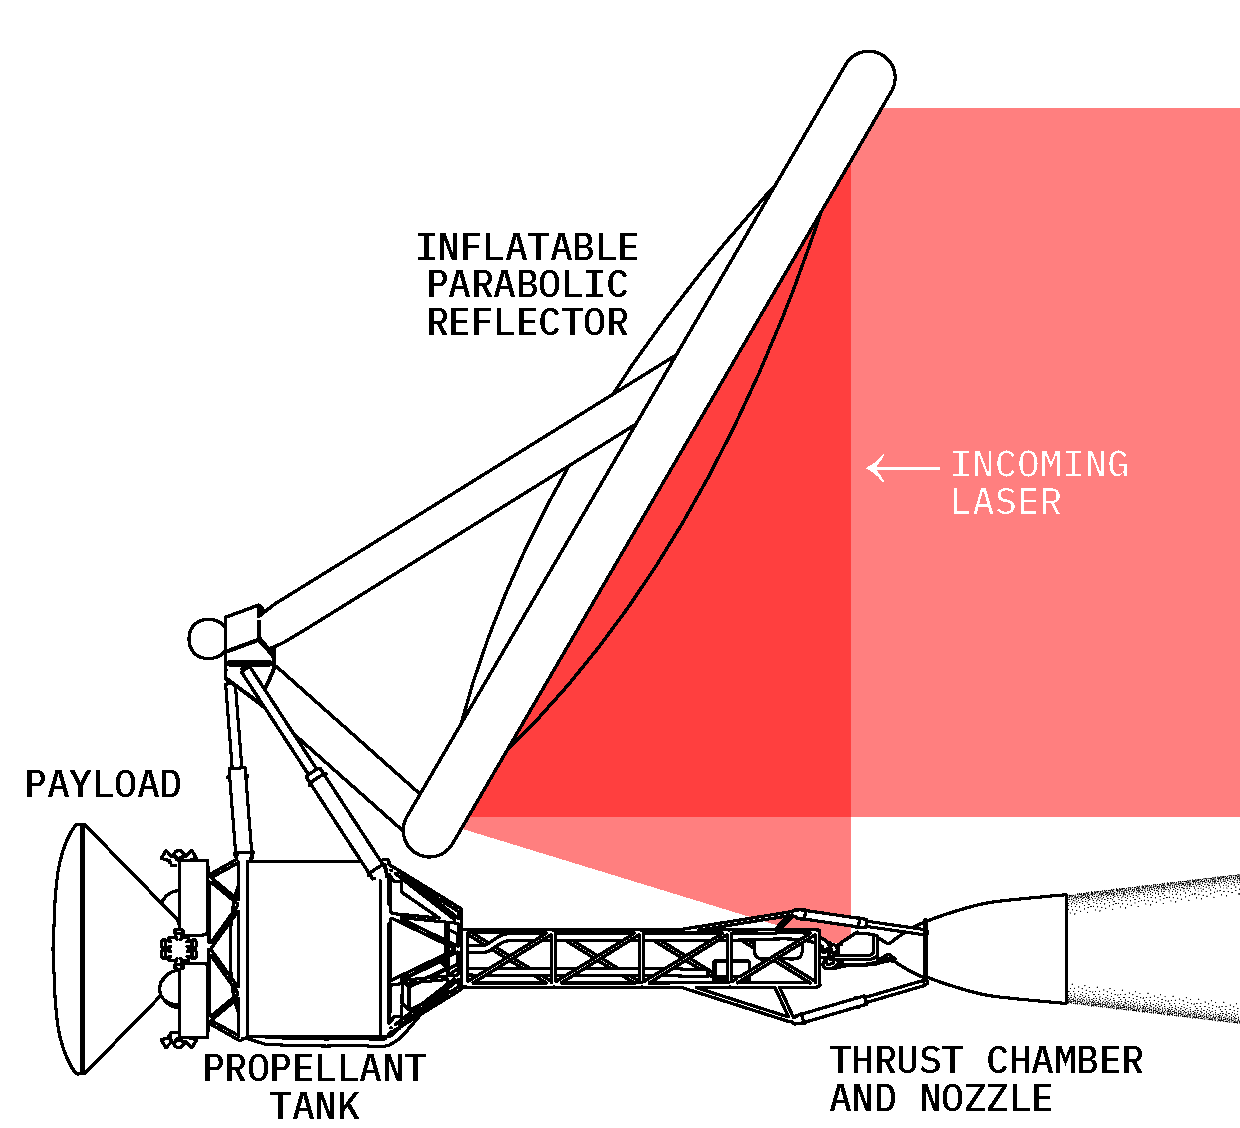
\includegraphics[width=\textwidth]{assets/2 background/overview_ltp}
                \caption{Spacecraft}
                \label{fig:overview_spacecraft}
            \end{subfigure}
            \begin{subfigure}[t]{0.64\textwidth}
                \centering
                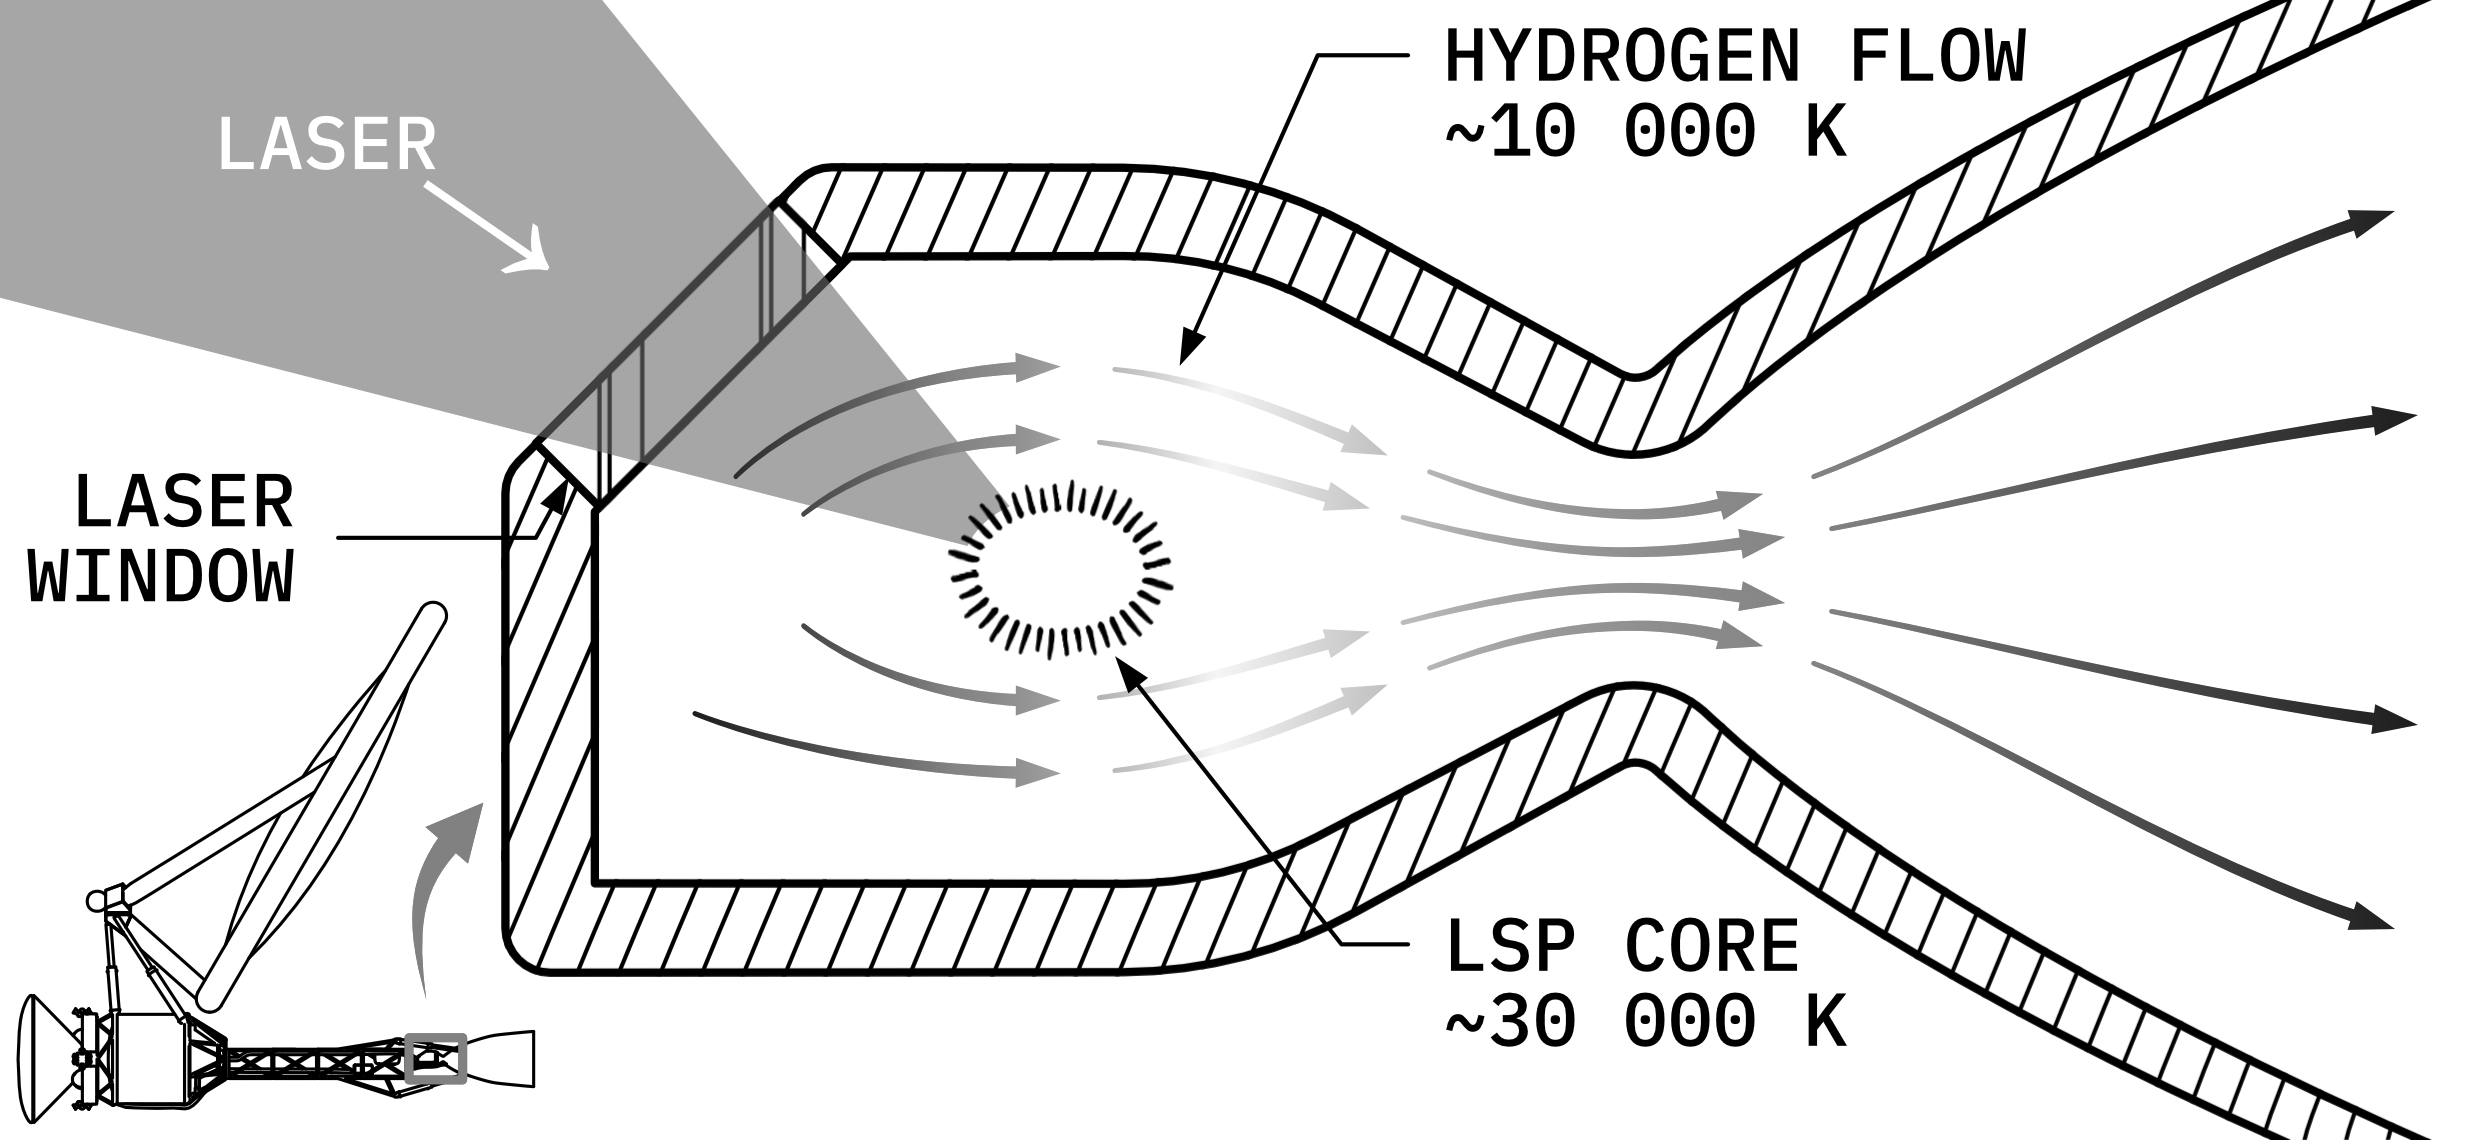
\includegraphics[width=\textwidth]{assets/2 background/chamber}
                \caption{Thrust chamber}
                \label{fig:overview_chamber}
            \end{subfigure}
            \caption[Overview of a CW laser-plasma LTP system]{Overview of a CW laser-plasma LTP system, adapted from \textcite{duplayDesignRapidTransit2022}}
            \label{fig:overview}
        \end{figure}

        As alluded to in the \nameref{chp:intro}, the key advantage of laser-thermal propulsion over chemical propulsion is its ability to deliver far greater exhaust velocities. Following from thermal rocket theory (\textcite{zandbergenAE4S01ThermalRocket2020}), the limiting exhaust velocity $v_\text{ex, max}$ of a thermal rocket motor depends on \autoref{eq:isp}, where $\gamma$ is the specific heat ratio of the propellant gas, $R_\text{u}$ is the universal gas constant, $\mathcal{M}$ is the propellant molar mass, and $T_\text{c}$ is the \added{bulk }chamber temperature.
        \begin{equation}
            I_\text{sp, max}g_0 = v_\text{ex, max} \propto \sqrt{2\frac{\gamma}{\gamma-1}\frac{R_\text{u}}{\mathcal{M}}T_\text{c}} \label{eq:isp}
        \end{equation}
        All other parameters being equal, a thermal rocket engine operating at a higher chamber temperature will thus have a greater limiting exhaust velocity.\added{ Chemical thrusters are fundamentally limited in their chamber temperature by the the adiabatic flame temperature of their propellants' chemical reaction. By comparison, an arbitrary amount of heat can theoretically be deposited via laser into a laser-thermal rocket engine (within thermal and structural limits).} By decoupling the thermal input from the propellant choice, a laser-thermal rocket engine can readily attain bulk temperatures of up to 10~000~K at the nozzle inlet, resulting in a specific impulse\footnote{Unless otherwise stated, values of specific impulse reported in this thesis refer to \emph{vacuum} specific impulse} of more than 1000~s with hydrogen propellant, as shown by \textcite{noredApplicationHighPower1976} in \autoref{fig:nored_Isp}.

        \begin{figure}[h]
            \centering
            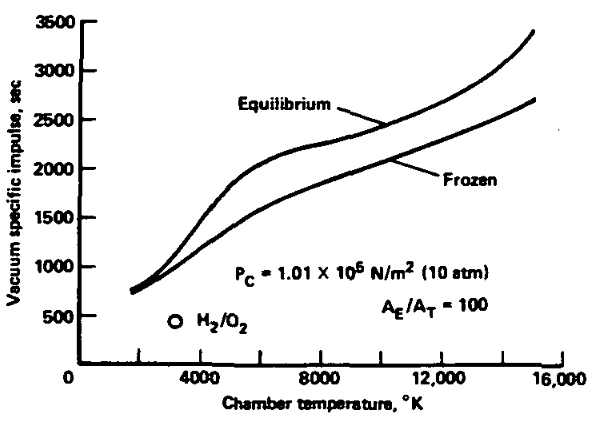
\includegraphics[width=0.7\textwidth]{assets/2 background/nored_ltpIsp.png}
            \caption[Theoretical specific impulse attained for a given hydrogen temperature]{Theoretical specific impulse attained for a given hydrogen temperature at the nozzle inlet, by \textcite{noredApplicationHighPower1976}. The specific impulse is bounded by two cases: 1.~the exhaust products maintain chemical equilibrium as they cool and expand through the nozzle; 2.~the composition of the exhaust is frozen}
            \label{fig:nored_Isp}
        \end{figure}

        Some practical issues with this concept do remain. Although it is well understood that the high propellant temperatures that could be achieved by LTP would result in \qtyrange{1000}{3000}{s} of specific impulse (with hydrogen), whether or not the heat deposited in the LSP can be transferred to all the propellant flow with minimal losses is a critical issue. This problem was studied in-depth by \textcite{shojiPerformanceHeatTransfer1976}, who performed a thorough analysis of heat transfer within two LTP engines, proposing seeding the flow with carbon particles as a solution to reduce radiative heat losses to the chamber walls. Their analysis showed that such losses could be reduced to 4.5\% of the input laser power for hydrogen seeded with 50\% carbon (by weight). While this is promising, such a system has yet to be tested experimentally. Furthermore, as suggested by \autoref{eq:isp}, the introduction of higher molar-mass carbon particles is associated with a penalty in the resulting specific impulse: \citeauthor{shojiPerformanceHeatTransfer1976}'s models show a decrease in theoretical specific impulse of around 25\%.

        Cooling is also an issue. Even with the inclusion of carbon seeding, the magnitude of laser power considered for DEP (MW to GW) makes 4.5\% of input power radiated to the thruster walls considerable. The propellant temperatures associated with high specific impulse are also far greater than the ones typically encountered by conventional thermal rocket engines, potentially necessitating new cooling strategies (\textcite{noredApplicationHighPower1976}). Thankfully, many of these cooling issues are similar in nature and magnitude to those encountered in Gas-Core Nuclear Rockets (GCNR), a sub-type of NTP. \textcite{kascakNozzleCavityWall1971} discusses a hydrogen GCNR operating at temperatures and specific impulses of the same order of magnitude, suggesting that a combination of transpiration cooling and gas seeding would be sufficient.

    \section{Laser-Sustained Plasma} \label{sec:background_lsp}
        One might wonder why bother with plasma at all. If the laser radiation could be deposited evenly in the propellant flow, little to no mixing would be needed and peak temperatures would be lower. Unfortunately, the use of lasers to directly heat \replaced{gaseous}{hydrogen} propellant has a major flaw: \replaced{the}{hydrogen} gas \replaced{might}{does} not absorb \replaced{the specific laser wavelength}{1-\unit{\um}-wavelength radiation} at room temperatures. \replaced{For instance, h}{H}ydrogen only begins to absorb \replaced{10.6-\unit{\um} radiation}{this wavelength} at around 10~000~K, as shown by \textcite{glumbConceptsStatusLasersupported1984}: ``The paradox is that hydrogen cannot absorb any laser radiation unless it is already hot.'' They were considering 10.6-\unit{\um} \deleted{laser }radiation\added{ emitted by \ce{CO2} lasers}, but this statement also holds for the 1.06-\unit{\um} \deleted{laser }wavelength\added{ emitted by fiber lasers}. This is because \highlight[id=ED]{these wavelengths do not match hydrogen's resonance absorption bands}, whereby radiation is absorbed in the rotational or vibrational modes of a molecule. \added{For instance, \textcite{campargueAbsorptionSpectrumH22011} show that there is a gap in the absorption bands of \ce{H2} in the 917--1090~nm range. }The main absorption mechanism in LSP is \emph{inverse bremsstrahlung} (IB): free electrons absorb radiation across a continuous spectrum (as opposed to specific wavelengths) during collisions with ions in the plasma (\textcite{keeferLaserSustainedPlasmas1989}). \textcite{johnstonCorrectValuesHighfrequency1973} showed that the radiation absorption coefficient $\alpha$ [\unit{m^{-1}}] can be calculated with \highlight[id=BZ, comment=It is not yet clear from this relation why the two wavelengths (...) would be improper to start up LSP (...)]{\autoref{eq:ib_absorption}}\comment[id=ED]{Clarified in-text}, where $Z$ is the ionic charge state (=1 for single-ionization), $n_\mathrm{e}$ is the electron density\added{ in \unit{cm^{-3}}}, $\nu$ is the radiation frequency, $k_\mathrm{B}$ is the Boltzmann constant, and $T_\mathrm{e}$ is the electron temperature in Kelvin.\added{ The product $k_\mathrm{B}T_\mathrm{e}$ should be expressed in \unit{eV}.} The Coulomb logarithm $\ln{\Lambda}$ and the plasma frequency $\nu_\mathrm{p}$ will be discussed in detail in \autoref{chp:models}.
        \newcommand{\ibalphaeq}{
            \alpha = \frac{7.8\times 10^{-7}Zn_\mathrm{e}^2\ln{\Lambda}}{\nu^2(k_\mathrm{B}T_\mathrm{e})^{3/2}} \left(1-\frac{\nu_\mathrm{p}^2}{\nu^2}\right)^{-1/2}\;[\unit{m^{-1}}]
        }
        \begin{equation}
            \ibalphaeq \label{eq:ib_absorption}
        \end{equation}
        \highlight[id=ED]{Since such free electrons are only present once gas has ionized} (i.e., $n_\mathrm{e} \gg \qty{0}{m^{-3}}$ ), absorption of 1.06-\unit{\um}-wavelength radiation can only occur in plasma by IB for gases that do not exhibit 1.06-\unit{\um} line transitions.

        While this negligible absorption at room temperature poses a problem to initiate the LSP process, \textcite{raizerSubsonicPropagationLight1970} theorized that once properly initiated, an LSP wave could be sustained in flowing gas. This was soon confirmed experimentally by \textcite{generalovContinuousOpticalDischarge1970}, who sustained a Xenon plasma using a 150-W CW \ce{CO_2} laser\added{ (i.e., 10.6-\unit{\um} wavelength)}. In addition to showing the feasibility of LSP, \citeauthor{generalovContinuousOpticalDischarge1970} also noted that the chamber pressure affects the ease of maintaining an LSP wave: in their experiments, they failed to maintain it below 3~\unit{atm}, and pressures above 4~\unit{atm} were too unstable\added{---the plasma had a tendency to die out. \citeauthor{generalovContinuousOpticalDischarge1970} gave no conclusive explanation of the phenomenon, suggesting only that combustion-instability effects could arise due to the asymmetry of the LSP observed beyond \qty{4}{atm}. Since later experiments have shown that this asymmetry is not a guarantee for instability, it is unclear whether other factors such as beam geometry (\citeauthor{generalovContinuousOpticalDischarge1970} used a low f-number of 1.25) were responsible for this observed instability. \textcite{zimakovInteractionNearIRLaser2016} reports stable Xenon plasmas sustained beyond \qty{20}{bar} with beam f-numbers ranging from 3 to 10.}

        Once a plasma is initiated, its shape and position will stabilize at an equilibrium point where the local laser intensity is just sufficient to compensate for thermal losses of the plasma front (\textcite{keeferLaserSustainedPlasmas1989}). This state and its stability will be affected by beam geometry and flow conditions (\textcite{welleEnergyConversionEfficiency1986}). Experiments by \textcite{fowlerIgnitionMaintenanceSubsonic1975} show that a key aspect of beam geometry is the ratio of the converging beam's focal length to its initial diameter at the focusing lens, known as the f-number, often denoted $f/N_\mathrm{f}$, where $N_\mathrm{f}$ is the f-number. Low f-numbers---i.e., short focal lengths with a wide initial beam diameter---produce stable plasmas which will remain close to the beam's focal point thanks to the rapid decrease in laser intensity, while the plasmas of high f-number optics will propagate away from the focus (\textcite{keeferLaserSustainedPlasmas1989}) and may be too unstable to be maintained continuously: \citeauthor{fowlerIgnitionMaintenanceSubsonic1975} have found that optical systems of $f/10$ and greater could not sustain a stable plasma.

        Since the first model derived by \citeauthor{raizerSubsonicPropagationLight1970}, theoretical/numerical models of LSP saw progressive improvements, providing greater insight into the optimal conditions for plasma maintenance and laser absorption. Notably, \textcite{jengNumericalStudyLasersustained1986} developed a fully two-dimensional numerical model of hydrogen LSP in 1986 that suggests close to complete laser absorption can be achieved under certain conditions (3~atm of static pressure, 10~kW input power). This model also showed that radial velocity components of the flow were significant, meaning that the one-dimensional or quasi-two-dimensional models developed earlier, such as the one by \textcite{battehTwoDimensionalGeneralization1974}, were unsuitable for the analysis of LSP problems. \citeauthor{jengNumericalStudyLasersustained1986}'s model also allowed for the study of the effect of the laser wavelength on the resulting plasma, an analysis that was impractical to perform experimentally. \citeauthor{jengNumericalStudyLasersustained1986} found that due to the gas absorption length's dependence on the applied electric field frequency, reducing the laser wavelength from \qtyrange{10.6}{3.9}{\um} led to lower absorption rates and longer plasmas along the beam axis, due to the inversely proportional relation seen in \autoref{eq:ib_absorption} (\textcite{keeferLaserSustainedPlasmas1989}). This is a highly relevant factor to consider for an experiment looking to study LSP using modern fiber lasers operating at \qty{1.06}{\um}.

        Several experiments on LSP have been performed since \citeauthor{generalovContinuousOpticalDischarge1970}'s first plasmatron in 1970. Early studies explored the parameter space for the successful maintenance of LSP, with specific attention given to the ranges of pressures and laser power (threshold power) required. \textcite{moodyMaintenanceGasBreakdown1975} provides a thorough exploration of this parameter space for argon plasmas sustained by a 10.6-\unit{\um} laser, showing a $P \propto 1/p^2$ relation between the laser power $P$ and the gas pressure $p$ at $<10$~atm, as shown in \autoref{fig:4_moodyArgon}. In his study, the minimum pressure at which an LSP was achieved was 2~atm, for a laser power approaching 300~W. Higher pressures allow for a lower input power and can enable ambient atmosphere operation of a thruster, greatly simplifying experimental design. Similar experiments performed for other gases showed that the threshold power was typically greater for molecular gases (e.g.,  hydrogen) (\textcite{keeferLaserSustainedPlasmas1989}).

        Another parameter affecting successful LSP maintenance is flow velocity, as shown by the studies of \textcite{welleEnergyConversionEfficiency1986,krierContinuousWaveLaser1986,gerasimenkoLaserPlasmatron1983}. While early experiments were typically performed in static gas, with natural convection being the only source of flow, the effect of forced convective flow was studied both for its benefits to the resulting LSP, and the application of LSP within a laser-thermal thruster. \citeauthor{welleEnergyConversionEfficiency1986} varied the flow speed from \qtyrange{0.4}{4.5}{m/s} in argon plasmas sustained by a 1~kW laser, measuring laser absorption and thermal radiation losses. They found that there are optimal pressure and flow speed conditions to maximize laser absorption, and that thermal radiation correlates with laser absorption. For pressures above 1.5~atm, increased flow speed appears to improve absorption compared to the static case. The authors suggest that the flow forced the plasma closer to the high-intensity laser focus, as seen in \autoref{fig:4_LSPTProfile}, improving absorption characteristics. In the case of \autoref{fig:4_LSPTProfile}, this translated to an improvement from 66\% to 83\%. \citeauthor{gerasimenkoLaserPlasmatron1983} found that in some cases, forced convection enables the maintenance of LSP under pressure and laser power conditions that would otherwise not allow it.

        \begin{figure}[h]
            \centering
            \begin{subfigure}[t]{0.50\textwidth}
                \centering
                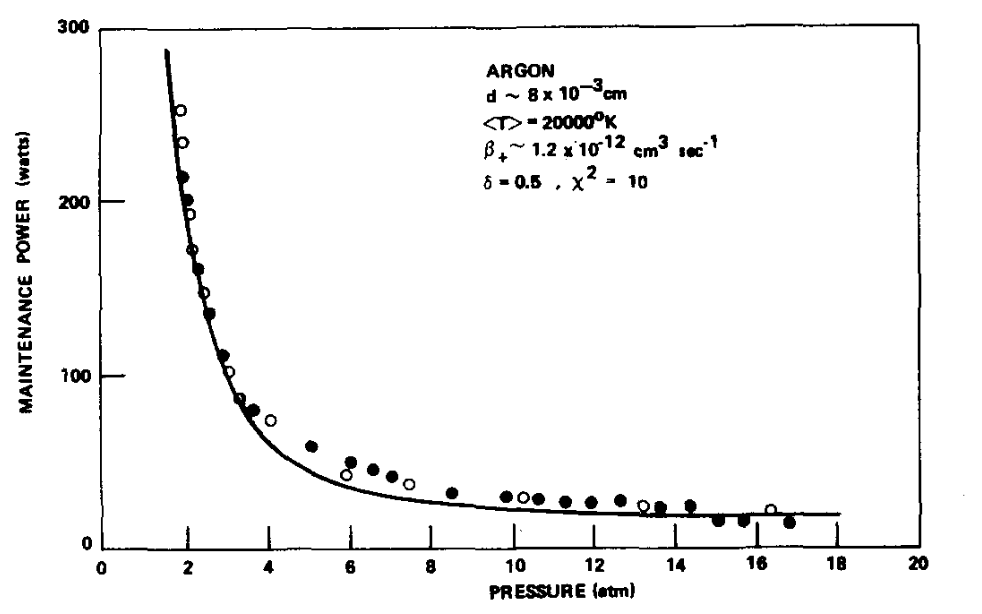
\includegraphics[width=\textwidth]{assets/2 background/moody_ArgonLSP.png}
                \caption[Pressure dependence on required laser input power to maintain LSP in argon]{Pressure dependence on required laser input power to maintain LSP in argon, reproduced from \textcite{moodyMaintenanceGasBreakdown1975}}
                \label{fig:4_moodyArgon}
            \end{subfigure}
            \hfill
            \begin{subfigure}[t]{0.45\textwidth}
                \centering
                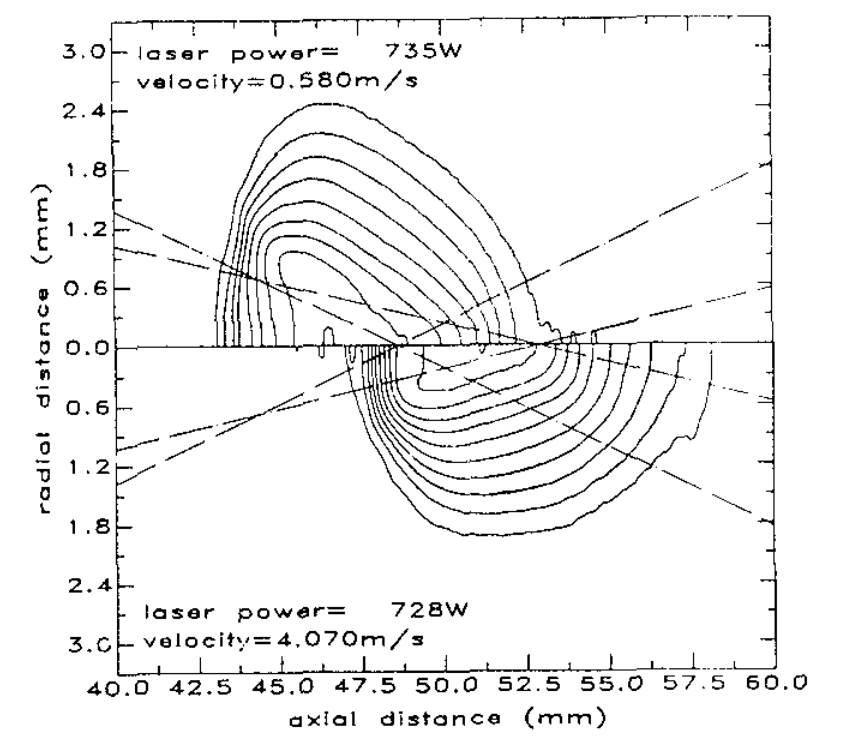
\includegraphics[width=\textwidth]{assets/2 background/welle_TProfile.png}
                \caption[Temperature profile of argon plasmas at two flow velocities]{Temperature profile of argon plasmas at two flow velocities, reproduced from \textcite{welleEnergyConversionEfficiency1986}. Intervals of 500~K with outer contour at 10~500~K.}
                \label{fig:4_LSPTProfile}
            \end{subfigure}
            \caption{Dependence of LSP on pressure and flow velocity}
            \label{fig:4_conditions}
        \end{figure}

    \section{Past facilities} \label{sec:background_exp}
        LSP and LTP experiments have been performed since the 1970s, with the very first LSP achieved by \textcite{generalovContinuousOpticalDischarge1970}, who used a \ce{CO_2} laser operating at \qty{10.6}{\um} to sustain a Xenon LSP. The use of \ce{CO_2} lasers is common in the literature that followed, although the optical setups, diagnostics, working gases, and configurations of LSP and LTP experiments vary greatly. Facilities from three research groups will be discussed in particular, for their significant published research output and relevance to propulsion applications: the facility at the University of Illinois (late 1980s), at the University of Tennessee (late 1980s), and in Japan, where LSP experiments were performed as recently as 2019. 

        \begin{figure}[h]
            \centering
            \begin{subfigure}[b]{0.55\textwidth}
                \centering
                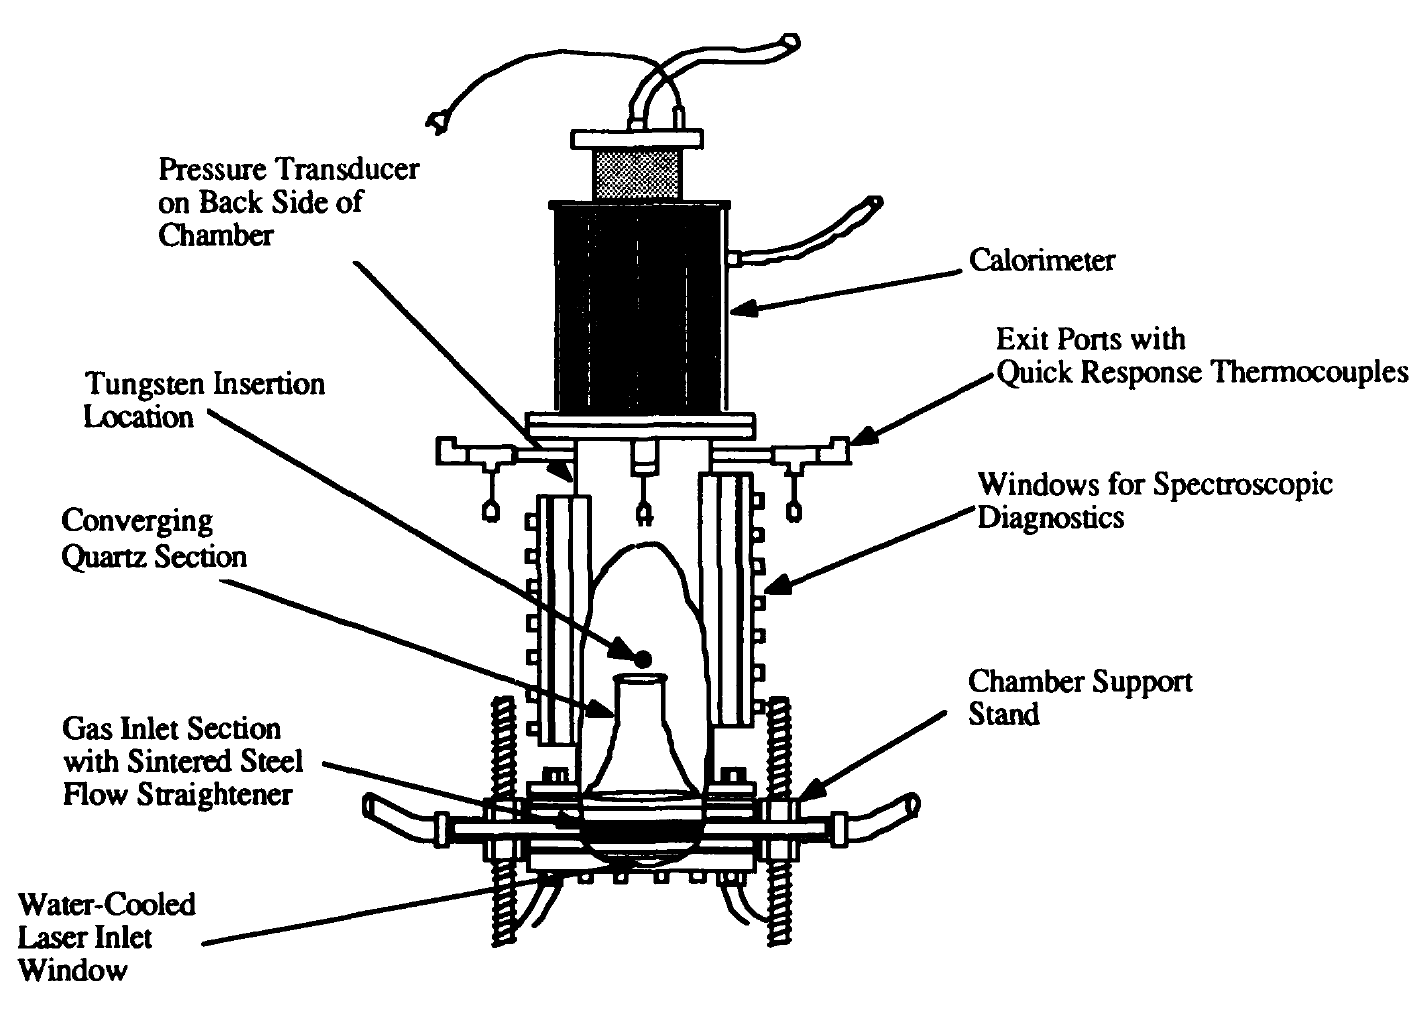
\includegraphics[width=\textwidth]{assets/2 background/uiuc_setup2.png}
                \caption{UIUC LSP experiment \cite{krierEnergyConversionMeasurements1988}.}
                \label{fig:4_uiucLSP}
            \end{subfigure}
            \hfill
            \begin{subfigure}[b]{0.43\textwidth}
                \centering
                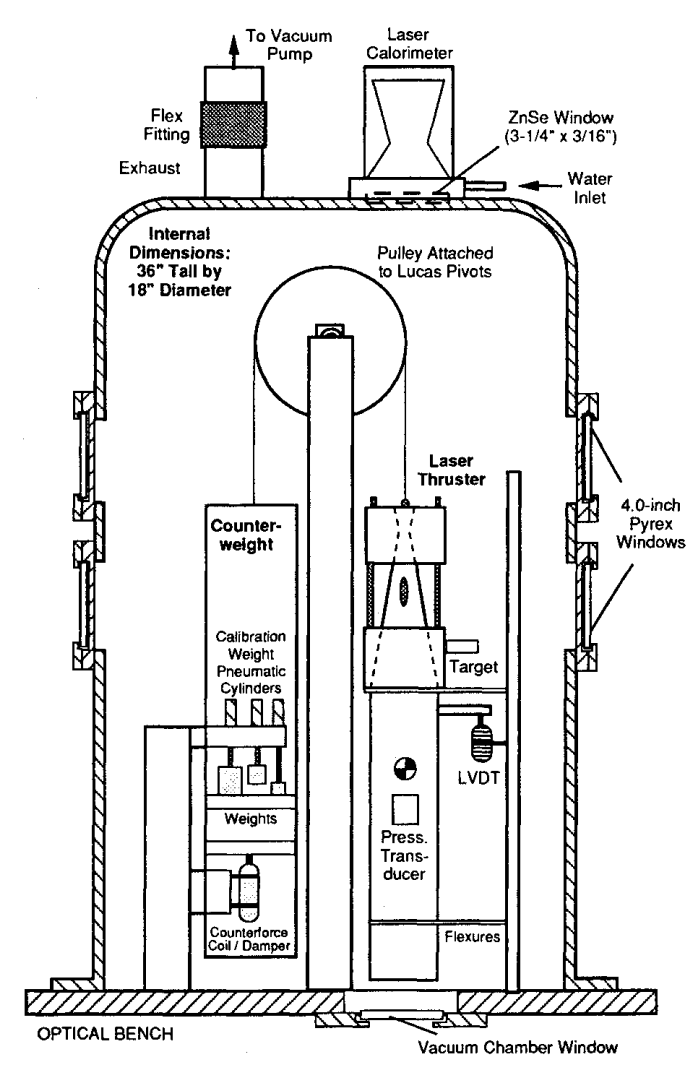
\includegraphics[width=\textwidth]{assets/2 background/uiuc_thrustStand.png}
                \caption{Thruster and thrust stand \cite{blackLaserPropulsion10kW1995}}
                \label{fig:4_uiucThrust}
            \end{subfigure}
            \caption{UIUC experimental configurations}
            \label{fig:4_uiuc}
        \end{figure}
        

        \subsection{University of Illinois Urbana-Champaign (UIUC)}
            This facility (depicted in \autoref{fig:4_uiucLSP}) was operated principally by Krier and Mazumder and was designed to characterize the energy conversion ability of LSPs, using argon as a working fluid in most cases. According to \textcite{schwartzLasersustainedGasPlasmas1989}, the LSP was sustained using a \ce{CO_2} laser with a maximum power of \qty{10}{kW}. The beam was focused into the absorption chamber with an elaborate set of reflective optics that allowed the maintenance of dual-plasma geometry, which was thought to reduce radiative losses and improve heat retention. Initiation of the plasma was achieved using a tungsten rod as a solid target, which was removed directly after plasma initiation using a solenoid actuator. The working fluid was argon for most experiments, at \qtyrange{1.0}{2.7}{atm} of gauge pressure. The absorption chamber design features devices to straighten and accelerate gas flow upstream of the LSP, facilitating the maintenance of a plasma at high flow rates, as turbulent flow were prone to blow out the plasma. These design features include a flow straightener as the gas inlet section, and a converging quartz nozzle, which enabled the acceleration of the chamber flow without the need to manufacture a narrower thrust chamber, as the facility was initially designed for low flow speeds ($< 2$~m/s) (\textcite{krierEnergyConversionMeasurements1988}). Most of their experiments revolved around laser absorption and thermal radiation, with little interest in thrust characteristics, so the heated gas exhaust was simply fed through exit ports. Nevertheless, experiments at this facility eventually led to the design and operation of a 10-kW-class thruster by \textcite{blackLaserPropulsion10kW1995}, with a 15:1 expansion ratio nozzle, achieving a specific impulse of up to 350~s, efficiencies near 40\%, and thrust exceeding 3~N using hydrogen propellant. In their study, efficiency $\eta$ is the thrust efficiency, calculated using \autoref{eq:thrust_efficiency}, based on a mass flow rate $\dot{m}$, thrust force $F_\mathrm{T}$, and laser power entering the thruster $P_\mathrm{in}$.
            \begin{equation} \label{eq:thrust_efficiency}
                \eta = \frac{F_\mathrm{T}^2}{2\dot{m}P_\mathrm{in}}
            \end{equation}
            Their thrust stand, like their LSP experiments, used a vertical configuration with a pulley and counterweight. The entire stand was encapsulated in a vacuum chamber. Thrust measurements were performed using  a combination of a linear variable differential transformer, which senses the displacement of the thruster, and a counterforce coil, which uses the detected displacement and attempts to counteract it. The current supplied to the coil can be correlated to the thrust force $F_\text{T}$. This force could then be used with a mass flow rate $\dot{m}$ measured with mass flow meters to compute specific impulse $I_\text{sp}$ with \autoref{eq:ispcalc}, which follows from thermal rocket theory.
            \begin{equation}
                I_\text{sp} = \frac{F_\text{T}}{\dot{m}g_0}
                \label{eq:ispcalc}
            \end{equation}

        \subsection{University of Tennessee Space Institute (UTSI)}
            The UTSI experiments were run using a 1.5-kW-class \ce{CO_2} laser. This facility is contemporary of the one at UIUC and shares similar design features, such as the vertical configuration and the converging gas inlet. Both facilities' absorption chambers are made in large parts out of quartz walls to allow for spectroscopic measurements to determine a spatial temperature distribution. In experiments performed by \textcite{keeferPowerAbsorptionLasersustained1986}, argon was used as the working fluid, at pressures ranging from \qtyrange{1.3}{2.3}{atm}, and laser powers as low as 360~W. A significant feature of their facility is the presence of a specialized laser beam dump integrated within the converging exit nozzle.

            \begin{figure}[h]
                \centering
                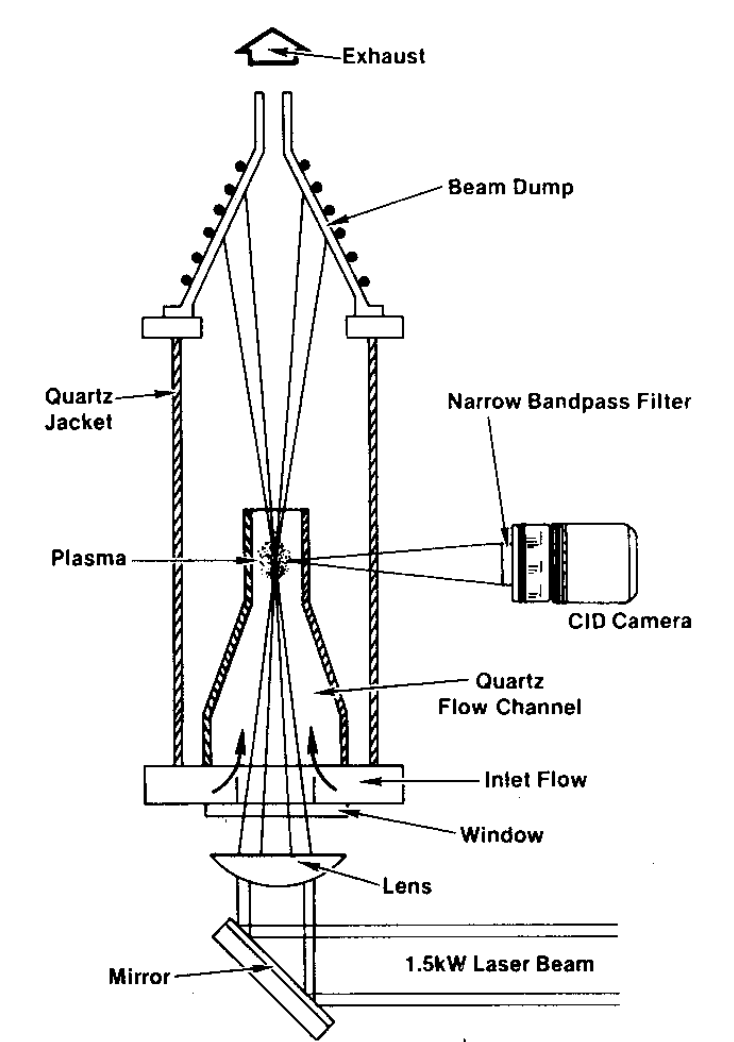
\includegraphics[width=0.5\textwidth]{assets/2 background/utsi_facility.png}
                \caption[UTSI LSP apparatus]{UTSI LSP apparatus \cite{keeferPowerAbsorptionLasersustained1986}}
                \label{fig:4_utsiExp}
            \end{figure}

        \subsection{Japanese experiments}
            The most recent LSP experiments have been performed at the University of Tokyo and Shizuoka University, studying not only the characteristics of LSP (\textcite{inoueOscillationPhenomenonLasersustained2004}), but also investigating its propulsion performance and its applications for replicating atmospheric re-entry conditions in wind tunnels (\textcite{matsuiAtomicOxygenFlowGenerationLaserDriven2014}). The Japanese facility (illustrated in \autoref{fig:4_tokyoThrust}) took a different approach to that of UIUC and UTSI, opting for a horizontally configured thrust stand. Instead of running the entire thruster within a vacuum chamber, the nozzle was connected to a separate vacuum tank by means of an expansion joint\added{, labelled Bellows in \autoref{fig:4_tokyoThrust}}. This \added{joint} allowed the thruster to exhaust to vacuum conditions with reduced complexity and without preventing the thruster from applying a force to the load cell\added{, as would be the case with a rigid connection to the vacuum tank}. The Tokyo research group performed experiments using a variety of working gases, laser powers, and plasma initiation methods. \textcite{matsuiGeneratingConditionsArgon2019} even performed experiments with disk, fiber, and diode lasers, a major change from the traditional use of \ce{CO_2} lasers. \added{In addition to emitting wavelengths of 1030, 1070, and \qty{940}{nm}, respectively, these lasers also offer improved energy efficiency, more compact form-factors, and easier maintenance compared to \ce{CO2} lasers (\textcite{matsuiGeneratingConditionsArgon2019})---all relevant factors for the development of DEP and LTP. These advantages do come at the cost of reduced IB absorption coefficients at comparable pressures, as discussed by \citeauthor{matsuiGeneratingConditionsArgon2019}.}

            \begin{figure}[h]
                \centering
                \begin{subfigure}[t]{0.60\textwidth}
                    \centering
                    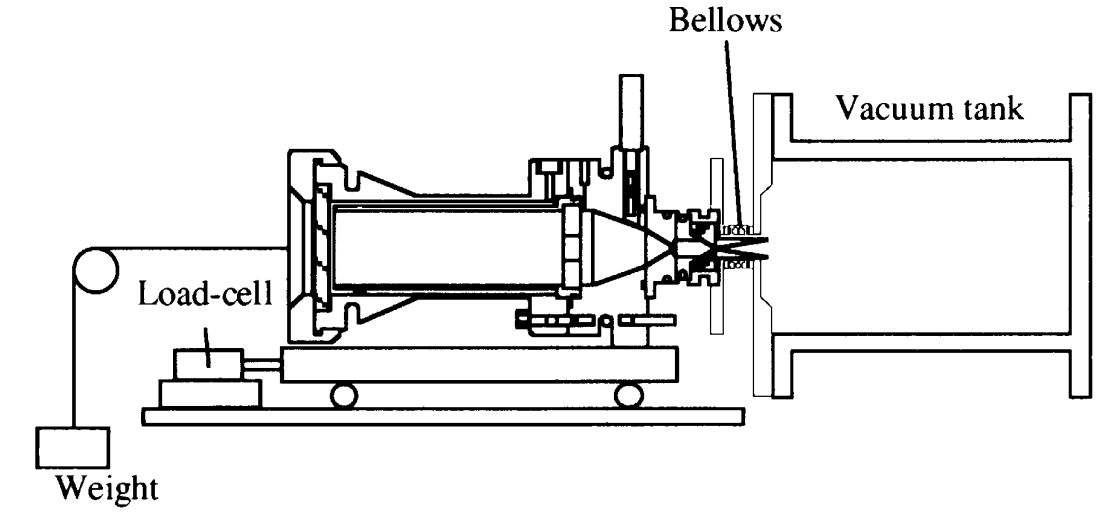
\includegraphics[width=\textwidth]{assets/2 background/tokyo_thrust.png}
                    \caption{Thrust measurement \cite{toyodaThrustPerformanceCW2002}}
                    \label{fig:4_tokyoThrust}
                \end{subfigure}
                \hfill
                \begin{subfigure}[t]{0.35\textwidth}
                    \centering
                    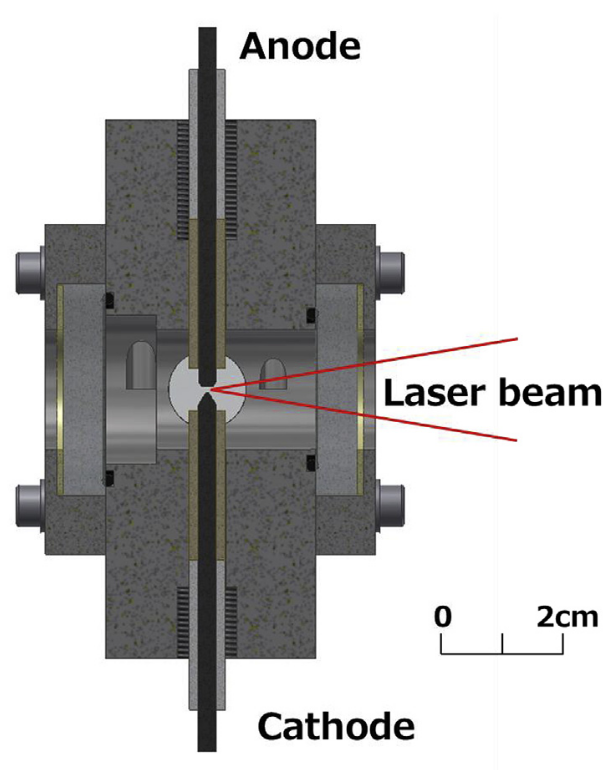
\includegraphics[width=\textwidth]{assets/2 background/tokyo_arc.png}
                    \caption{LSP initiation through arc discharge \cite{matsuiGeneratingConditionsArgon2019}}
                    \label{fig:4_tokyoArc}
                \end{subfigure}
                \caption{University of Tokyo LSP apparatus}
                \label{fig:4_tokyo}
            \end{figure}

            The Japanese LSP chambers generally follow a similar design as those of UIUC and UTSI, i.e., a cylindrical section followed by a converging-diverging nozzle. However, they do not feature some of the additional flow control devices seen in the other facilities, such as the converging gas inlet channel. Instead, it appears many of their LSPs are maintained just downstream of the cylindrical section, which then allows the flow to naturally develop before it reaches the plasma. The gas inlet is also placed close to the nozzle, forcing the gas to flow between the internal and external walls of the thruster before entering the main chamber near the laser window, acting as a regenerative cooling system. \added{The LSP's axial position could be controlled by moving the laser focusing lens using a one-axis stage. }The thruster also features a two-stage converging nozzle, with a sub-chamber in which the LSP is moved to after initiation, resulting in improved thrust levels (\textcite{toyodaThrustPerformanceCW2002}). This is likely due to the improved absorption ability of LSP at higher flow speeds observed by \textcite{welleEnergyConversionEfficiency1986}.

            The thrust measurement method used by \textcite{toyodaThrustPerformanceCW2002} is also considerably simpler than the implementation used by \textcite{blackLaserPropulsion10kW1995}. The thruster is mounted on low-friction linear rails and placed in contact with a load-cell. Weights on a pulley are used to balance the initial loads on the thruster. When operating the thruster to vacuum exhaust, the spring constant of the expansion joint was taken into account and compensated for. Furthermore, the motor was first run as a cold-gas thruster, using this initial thrust level as a reference to quantify the effect of the LSP. Efficiency was measured differently than in UIUC experiments, using \autoref{eq:japan_thrustefficiency}~\cite{toyodaThrustPerformanceCW2002}\footnote{The cited reference appears to have a typographical error, as the units are inconsistent. This equation can be derived from the conventional thrust efficiency equation, assuming a constant mass flow rate.}, to separate the effect of the LSP from the baseline cold thrust $F_\text{T, cold}$. This provides a more meaningful measurement of the energy-conversion efficiency of LSP for propulsion applications.
            \begin{equation} \label{eq:japan_thrustefficiency}
                \eta = \frac{F_\text{T, hot}^2-F_\text{T, cold}^2}{2\dot{m}P_\mathrm{in}}
            \end{equation}

            Two methods of plasma initiation were used throughout their experiments. Early thruster studies used a tungsten rod in the same manner as \textcite{schwartzLasersustainedGasPlasmas1989} at UIUC. A later study by \textcite{matsuiGeneratingConditionsArgon2019} used an arc discharge at the laser focus point, seen in \autoref{fig:4_tokyoArc}. This solid-state method of plasma initiation is attractive for its mechanical simplicity and its ability to quickly react to control inputs compared to solenoid-actuated ignition rods.

        \subsection{Other LSP facilities}
            In addition to the LTP experiment described above, two recent experimental studies are considered for comparison with this project: those of \textcite{zimakovInteractionNearIRLaser2016,luCharacteristicDiagnosticsLaserStabilized2022}, pictured in \autoref{fig:recentLSPsystems}. While they do not study LSP for thrust applications, they are of interest as they are some of only a few experiments using \num{1.06}-\unit{\um}fiber lasers to sustain plasma in argon, like in this project. In addition, both experiments appear to successfully use an arc discharge for LSP ignition, which differs from much of the older experimental literature.

            \begin{figure}[h]
                \centering
                \begin{subfigure}[t]{0.47\textwidth}
                    \centering
                    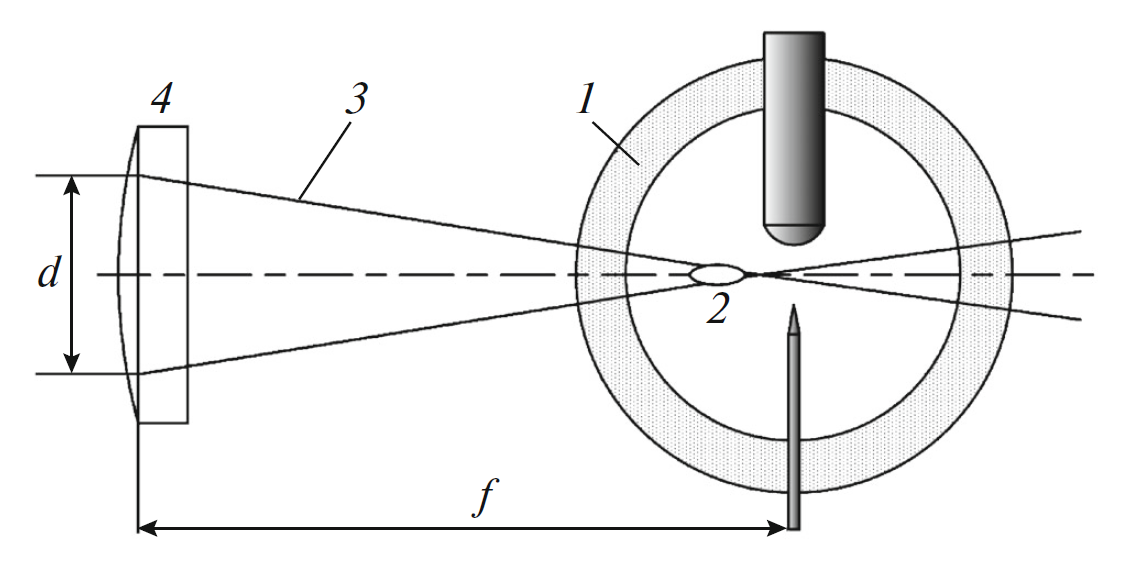
\includegraphics[width=\textwidth]{assets/2 background/zimakov.png}
                    \caption{\textcite{zimakovInteractionNearIRLaser2016} (2016): (1) pressurized bulb, (2) LSP, (3) laser beam boundaries, (4) lens with focal length $f$}
                    \label{fig:recentLSPsystems_zimakov}
                \end{subfigure}
                \hfill
                \begin{subfigure}[t]{0.47\textwidth}
                    \centering
                    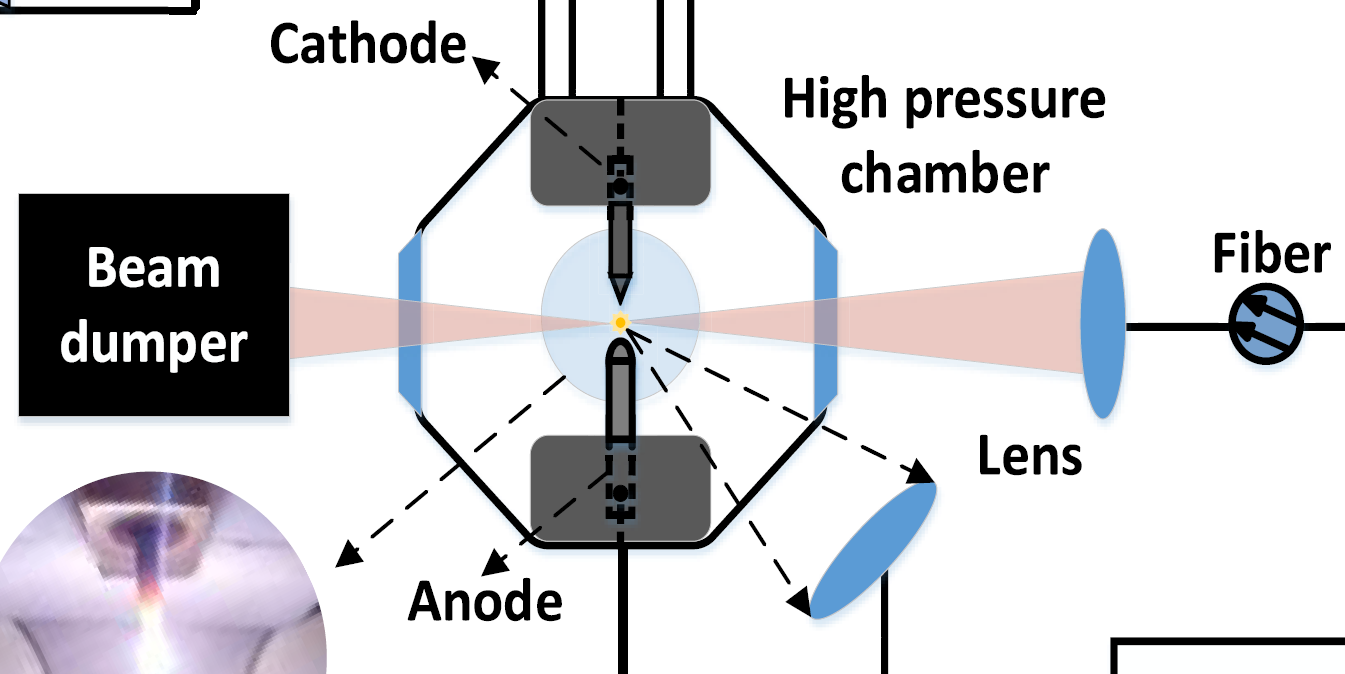
\includegraphics[width=\textwidth]{assets/2 background/LuYuanSongetal.png}
                    \caption{\textcite{luCharacteristicDiagnosticsLaserStabilized2022} (2022)}
                    \label{fig:recentLSPsystems_lu}
                \end{subfigure}
                \caption{Recent argon LSP generator designs}
                \label{fig:recentLSPsystems}
            \end{figure}

            \textcite{zimakovInteractionNearIRLaser2016}'s investigation focuses on determining the power necessary to sustain a steady argon and Xenon LSP, providing a simple model to plot this power threshold in terms of gas pressure, using experimentally determined parameters. Comparing their power threshold data with that of \textcite{moodyMaintenanceGasBreakdown1975} shows a drastic increase in required laser power for similar pressures, going from around \qtyrange{50}{1000}{W} at \qty{6}{bar}, due to the change of laser wavelength from \qtyrange{10.6}{1.07}{\um}. This can be expected due to the reduced IB absorption coefficient, as seen in \autoref{eq:ib_absorption} \added{and \autoref{fig:alphadiff}}. They also attempt to determine plasma temperature by comparing the continuum emission spectrum of the LSP with the predicted spectrum of a plane slab plasma of comparable dimensions, approximating the LSP temperature to be \qty{15000}{K} for laser powers ranging from 65 to \qty{230}{W} at \qty{22}{bar}.

            \begin{figure}[h]
                \centering
                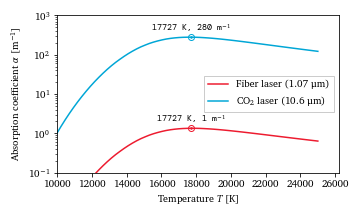
\includegraphics[]{assets/2 background/alphadiff}
                \caption[IB absorption coefficient for \ce{CO2}- and fiber-laser radiation]{IB absorption coefficient at \qty{1}{bar} for \ce{CO2}- and fiber-laser radiation}
                \label{fig:alphadiff}
            \end{figure}

            \textcite{luCharacteristicDiagnosticsLaserStabilized2022} performed in-depth spectroscopic analysis to determine plasma parameters, namely temperature and electron density. By using a line-to-continuum spectral analysis method, they estimated the LSP temperature to be \qty{13000}{K} (\qty{13}{bar}, \qty{200}{W}).

    \section{Takeaways and research objectives}
        Research on LTP and LSP, beginning in the 1970s, suggest that LTP has a great potential as a high-efficiency, high-thrust propulsion concept with performance rivaling that of NTP systems.\added{ The use of ground-based laser arrays to transmit power virtually eliminates the power-generation subsystem mass from a spacecraft, enabling it to perform high-delta-$v$ maneuvers in a shorter timespan than equivalent systems using on-board power.} Although concerns regarding laser tracking, thrust chamber cooling, and engine efficiency present engineering challenges, no fundamental issues have been identified. Extensive literature on LSP sustained by \ce{CO_2} lasers exists and have shown promising results in terms of laser absorption by the LSP, one of the major potential loss factors for an LTP system: very high absorption was experimentally achieved under a variety of conditions. On the other hand, heat deposition from the LSP into the surrounding cold propellant is far less efficient, but potential solutions have been proposed, such as seeding the propellant flow with carbon or tungsten particles to improve radiative absorption.

        LTP thruster laboratory models have been operated, but not since the early 2000s, never with fiber lasers, and some of the radiative absorption strategies mentioned earlier have yet to be tested to improve thrust efficiency. Recent research has nevertheless begun experimenting with \replaced{argon LSP powered by fiber-lasers, which offer the modularity required to construct DEP laser arrays}{fiber-laser-powered LSP, namely with argon}, but not for propulsion applications. They have demonstrated the feasibility of LSP using such lasers, with peak temperatures on the same order of magnitude as those sustained by \ce{CO_2} lasers, although the necessary power required was approximately an order of magnitude greater, due to the lower absorption coefficient predicted by IB theory. There is still lacking experimental work on the resulting heat deposition into the working gas from the LSP, a critical metric for thruster design, as this heat should ideally be retained in the exhausted propellant to maximize jet power and thrust efficiency.

        Considering the current context of directed-energy propulsion favoring fiber lasers operating at \qty{1.06}{\um} rather than the \ce{CO_2} lasers historically considered for LTP, there is a rationale to pursue and update research on LTP and LSP at a fiber laser wavelength. This is \emph{despite} the less favorable IB absorption characteristics at this wavelength. With the long-term objective of developing fully-fledged LTP experimental capabilities at McGill University, the following near-term research objectives were set for this project:
        \begin{enumerate}
            \item Build an argon LSP generator/thruster model to replicate the results of recent, comparable experiments (\cite{matsuiGeneratingConditionsArgon2019,zimakovInteractionNearIRLaser2016,luCharacteristicDiagnosticsLaserStabilized2022}) \\
                \textit{Rationale: This establishes a baseline that can be validated against the literature.}
            \item Determine heat deposition from the LSP into the working gas \\
                \textit{Rationale: Understanding the resulting heat deposition can be used to predict thruster performance and/or optimize an LTP thruster using conventional thermal rocket theory.}
        \end{enumerate}
        \added{For this project, argon was selected as a working fluid rather than hydrogen. This is in most part due to its safer handling characteristics compared to hydrogen. It also has a lower ionization energy~\cite{kramidaNISTAtomicSpectra2022} than neon (a lighter inert gas), is affordable, and its monatomic nature simplifies thermodynamic calculations since no dissociation can occur. Future studies following this project are expected to use hydrogen, especially for thruster prototypes, as hydrogen's lower molecular weight is beneficial to maximize exhaust velocity.}